\documentclass{beamer}
\usetheme{Madrid}

\usecolortheme{default}
\useinnertheme{circles}
\usepackage[brazilian]{babel}
\usepackage{amsmath,mathtools,amsfonts,amssymb}
\usepackage{graphicx}
\usepackage[Algoritmo]{algorithm}
\usepackage{algpseudocode}

% Caminhos das imagens reutilizadas do LaTeX final da monografia
\graphicspath{{../}{../plots/}{../results/}}

% Redefine existing commands
\algrenewcommand\algorithmicwhile{\textbf{Enquanto}}
\algrenewcommand\algorithmicdo{\textbf{faça}}
\algrenewcommand\algorithmicif{\textbf{Se}}
\algrenewcommand\algorithmicthen{\textbf{então}}
\algrenewcommand\algorithmicelse{\textbf{senão}}
\algrenewcommand\algorithmicfor{\textbf{Para}}
\algrenewcommand\algorithmicforall{\textbf{Para todo}}
\algrenewcommand\algorithmicrepeat{\textbf{Repita}}
\algrenewcommand\algorithmicuntil{\textbf{até}}
\algrenewcommand\algorithmicprocedure{\textbf{Procedimento}}
\algrenewcommand\algorithmicfunction{\textbf{Função}}
\algrenewcommand\algorithmicreturn{\textbf{Retorne}}
\algrenewcommand\algorithmicend{\textbf{Fim}}

% Define new commands that don't exist by default
\algnewcommand\algorithmicendwhile{\textbf{fim enquanto}}
\algnewcommand\algorithmicendif{\textbf{fim se}}
\algnewcommand\algorithmicendfor{\textbf{fim para}}

\title[Detecção de Estados Operacionais]{Sistema de Detecção de Estados Operacionais de Equipamentos Industriais utilizando Machine Learning}
\subtitle{Trabalho de Conclusão de Curso}
\author[Felipe C. Lopes]{Felipe Costa Lopes \\ {\footnotesize Matrícula: 2018019648} \\ {\footnotesize Orientadora: Profa. Gabriela Nunes}}
\institute[UFMG]{Universidade Federal de Minas Gerais}
\date{\today}

\begin{document}

% ===================== CAPA =====================
\begin{frame}
    \titlepage
\end{frame}

% ===================== AGENDA =====================
\begin{frame}{Roteiro}
    \tableofcontents
\end{frame}

% =====================================================================
\section{Introdução}
% =====================================================================

% Slide: Contextualização
\begin{frame}{Contextualização: equipamentos ``caixa preta''}
    \begin{columns}
        \column{0.5\textwidth}
        \textbf{Situação real:}
        \begin{itemize}
            \item Muitos equipamentos operam como ``caixas pretas''.
            \item O estado real (ligado/desligado) não chega à infraestrutura IoT.
        \end{itemize}

        \column{0.5\textwidth}
        \textbf{Consequências:}
        \begin{itemize}
            \item Ciclo operacional desconhecido.
            \item Indicadores de produção e manutenção imprecisos.
            \item Soluções tradicionais não escalam para a diversidade de plantas.
        \end{itemize}
    \end{columns}
\end{frame}

% Slide: Objetivo
\begin{frame}{Objetivo}
    \begin{block}{Meta principal}
        Detectar de forma \textbf{não invasiva} e \textbf{automática} os estados LIGADO/DESLIGADO usando sensores IoT \textbf{já instalados}.
    \end{block}
    \vspace{0.3cm}
    \textbf{Diferenciais:}
    \begin{itemize}
        \item \textbf{Agnóstico:} atende equipamentos elétricos e mecânicos.
        \item \textbf{Não supervisionado:} aprende os padrões sem rotulação manual.
        \item \textbf{Baixo custo:} reaproveita a infraestrutura IoT existente.
    \end{itemize}
\end{frame}

% Slide: Lição metodológica (CNN -> K-Means)
\begin{frame}{Por que aprendizado não supervisionado?}
    \textbf{Primeira tentativa: redes profundas (CNN / \textit{Autoencoders}).}
    \begin{itemize}
        \item Acurácia de treino aparente de 100\%, mas \textbf{não generalizavam}.
        \item Classificavam como LIGADO períodos com RPM\,=\,0 e corrente nula.
    \end{itemize}
    \vspace{0.3cm}
    \begin{block}{Lição}
        Problemas simples pedem soluções simples. Migrou-se para \textbf{K-Means}: robusto, interpretável, sem \textit{overfitting} e de treino rápido.
    \end{block}
\end{frame}

% Slide: Tecnologias
\begin{frame}{Tecnologias e ferramentas}
    \begin{itemize}
        \item \textbf{Linguagem:} Python 3.11+
        \item \textbf{Dados:} \textbf{InfluxDB} (séries temporais para IoT)
        \item \textbf{Processamento:} \textit{Pandas}, \textit{NumPy}, \textit{SciPy} (interpolação PCHIP/KNN)
        \item \textbf{\textit{Machine Learning}:} \textit{Scikit-learn} (K-Means, MinMax)
        \item \textbf{Interface:} \textit{CustomTkinter} (GUI para operadores)
        \item \textbf{Visualização:} \textit{Matplotlib} (gráficos 3D)
    \end{itemize}
\end{frame}

% =====================================================================
\section{Metodologia}
% =====================================================================

% Slide: Visão geral do pipeline
\begin{frame}{Visão geral do \textit{pipeline}}
    \begin{columns}
        \column{0.46\textwidth}
        \textbf{Pipeline dual e modular:}
        \begin{enumerate}
            \item Detecção automática do tipo (elétrico/mecânico).
            \item Coleta e segmentação.
            \item Interpolação e tratamento de \textit{outliers}.
            \item Sincronização e normalização.
            \item Classificação K-Means.
        \end{enumerate}
        \column{0.54\textwidth}
        \begin{center}
            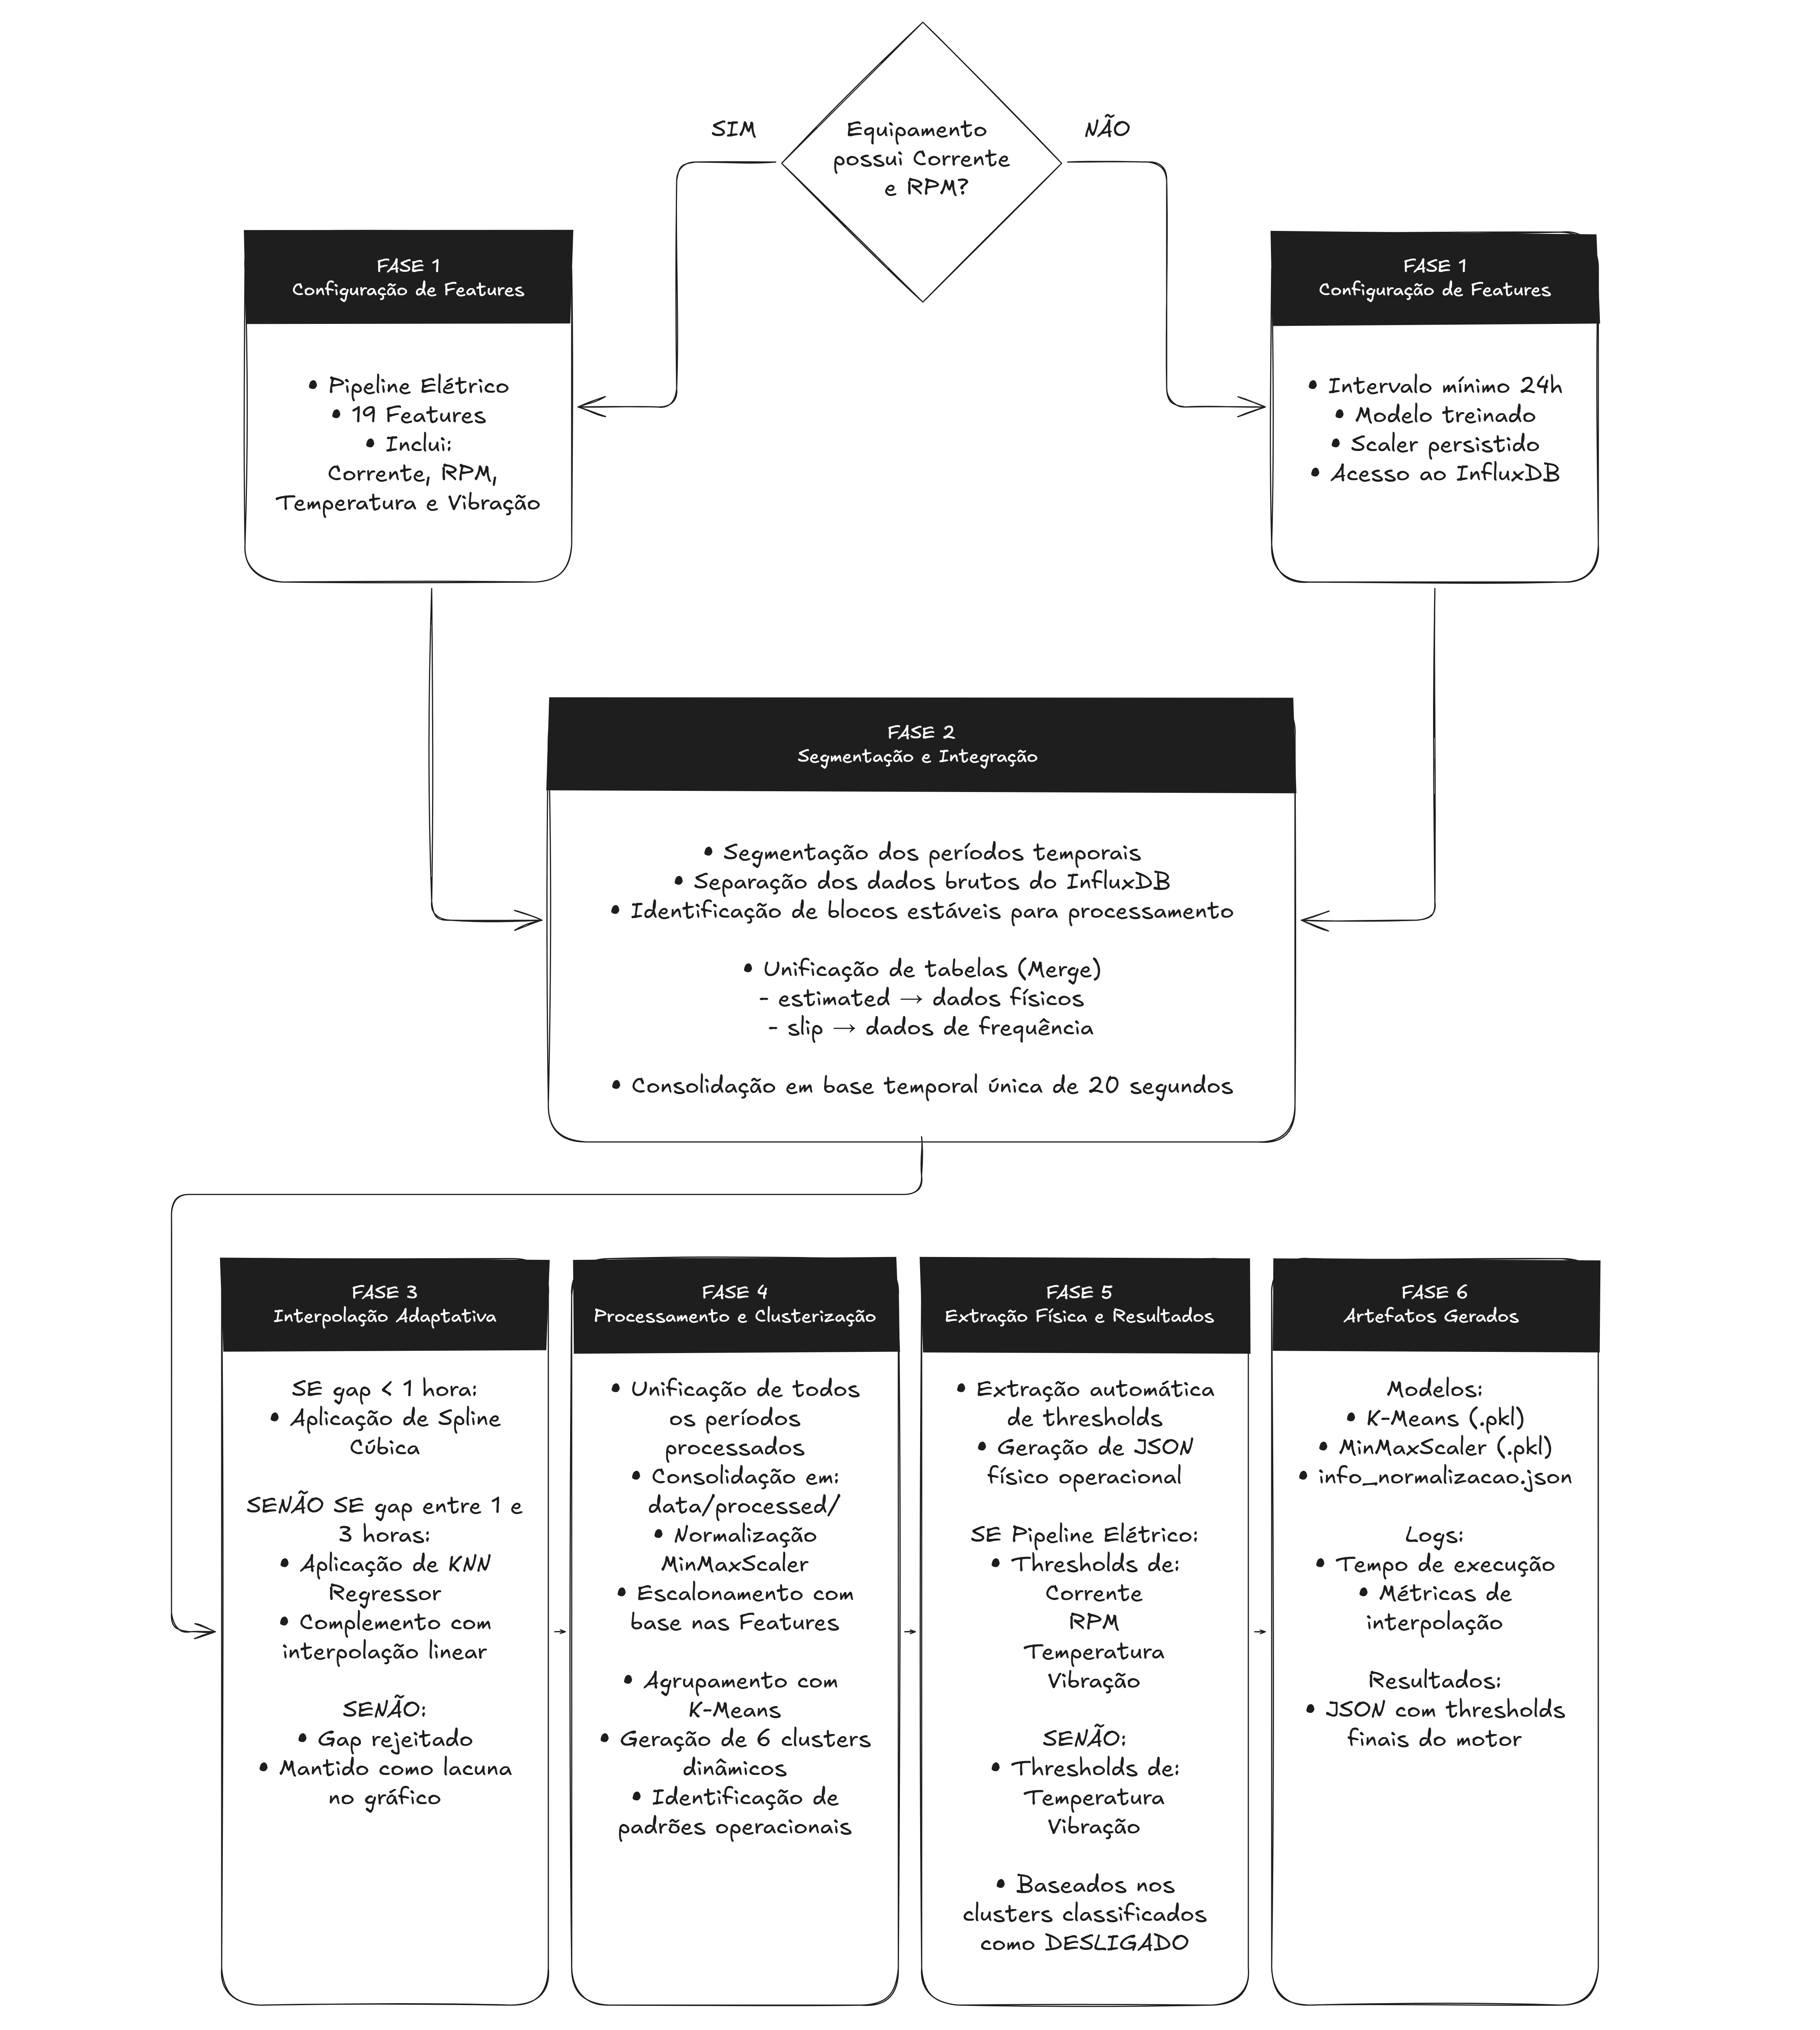
\includegraphics[height=0.78\textheight]{05_pipeline_treino.png}
        \end{center}
    \end{columns}
\end{frame}

% Slide: Coleta e segmentação
\begin{frame}{Coleta e segmentação temporal}
    \begin{itemize}
        \item \textbf{3 fontes (elétrico):} \texttt{validated\_default} (20\,s), \texttt{estimated} ($\sim$1\,min) e \texttt{validated\_slip} (2\,min). Mecânicos usam apenas 2.
        \item \textbf{Download} em \texttt{.csv} via \textit{script} Python a partir do InfluxDB.
        \item \textbf{Segmentação por lacunas:} \textit{gaps} $>$ 3\,h $\Rightarrow$ novos períodos independentes.
        \item Cada período válido recebe uma \textbf{linha temporal uniforme} (grade de 20\,em\,20\,s).
    \end{itemize}
\end{frame}

% Slide: Tratamento de outliers
\begin{frame}{Tratamento de \textit{outliers} (IQR)}
    \begin{columns}
        \column{0.42\textwidth}
        \begin{itemize}
            \item IQR com multiplicador conservador (3,0).
            \item Proteção de inércia: sequências $\geq$ 10 amostras são \textbf{preservadas} (não são ruído).
            \item Filtro anti-EMI: zera RPM/corrente espúrios (\textless\,2\,A).
        \end{itemize}
        \column{0.58\textwidth}
        \begin{center}
            
\includegraphics[width=\linewidth]{04_remocao_outliers.png}
        \end{center}
    \end{columns}
\end{frame}

% Slide: Interpolação adaptativa
\begin{frame}{Interpolação adaptativa de lacunas}
    \begin{columns}
        \column{0.42\textwidth}
        \textbf{Estratégia por tamanho:}
        \begin{itemize}
            \item $\leq$ 30\,min: \textbf{PCHIP} (sem oscilações de Runge).
            \item 30\,min--3\,h: \textbf{KNN} temporal + linear.
            \item $>$ 3\,h: \textbf{não interpola} (novo período).
        \end{itemize}
        \footnotesize LSTM testada, mas sem ganho frente ao KNN.
        \column{0.58\textwidth}
        \begin{center}
            
\includegraphics[width=\linewidth]{02_comparativo_knn_lstm_subplots.png}
        \end{center}
    \end{columns}
\end{frame}

% Slide: Normalização
\begin{frame}{Normalização robusta}
    \begin{columns}
        \column{0.42\textwidth}
        \begin{itemize}
            \item \textit{MinMax Scaler} para o intervalo $[0,1]$.
            \item \textit{Clipping} de \textit{outliers} no percentil 99,5\%.
            \item Preserva a forma e a distribuição; ajusta apenas a escala.
            \item Equilibra grandezas de escalas distintas.
        \end{itemize}
        \column{0.58\textwidth}
        \begin{center}
            
\includegraphics[width=\linewidth]{01_minmax_scaler.png}
        \end{center}
    \end{columns}
\end{frame}

% Slide: K-Means
\begin{frame}{O coração do sistema: K-Means}
    \begin{columns}
        \column{0.5\textwidth}
        \textbf{Por que não um limiar fixo?}
        \begin{itemize}
            \item Vibração residual de máquinas vizinhas.
            \item Variação da temperatura ambiente.
        \end{itemize}
        \vspace{0.2cm}
        \textbf{Configuração:}
        \begin{itemize}
            \item \textbf{k = 6} (proporção $\sim$1:2 entre desligado e ligado, captando transições).
            \item \textit{score} ponderado pela física.
        \end{itemize}
        \column{0.5\textwidth}
        \begin{center}
            
\includegraphics[width=\linewidth]{03_kmeans_animacao.png}
        \end{center}
    \end{columns}
\end{frame}

% Slide: Classificação ponderada (scores)
\begin{frame}{Classificação ponderada por física}
    \textbf{\textit{Score} de cada centróide:}
    \begin{align*}
        S_{\text{elétrico}}  &= 2{,}0\,\bar{C}_{\text{corr}} + 2{,}0\,\bar{C}_{\text{RPM}} + 1{,}0\,\bar{C}_{\text{vib}} + 0{,}5\,\bar{C}_{\text{temp}} \\
        S_{\text{mecânico}} &= 1{,}5\,\bar{C}_{\text{temp}} + 1{,}0\,\bar{C}_{\text{vib}} + 0{,}5\,\bar{C}_{\text{mag}}
    \end{align*}
    \begin{itemize}
        \item \textbf{Elétricos:} peso maior em corrente e RPM.
        \item \textbf{Mecânicos:} peso maior em temperatura e vibração.
        \item \textbf{Travas físicas:} \textit{hard rules} e \textit{Vibration Safety Floor} (vibração acima do piso $\Rightarrow$ LIGADO).
    \end{itemize}
\end{frame}

% Slide: Algoritmo (pseudocódigo)
\begin{frame}{Lógica de classificação dos \textit{clusters}}
    \begin{algorithm}[H]
        \caption{Classificação de estados via K-Means}
        \begin{algorithmic}[1]
            \Procedure{ClassificarEstados}{$X$ normalizado}
            \State Treinar K-Means com $k=6$ sobre $X$
            \For{cada centróide $c_i$}
            \State Calcular o \textit{score} ponderado $S_i$
            \EndFor
            \State Ordenar \textit{clusters} por $S_i$ crescente
            \State \textit{Cluster} de menor \textit{score} $\rightarrow$ DESLIGADO
            \For{demais \textit{clusters}}
            \If{vibração $>$ piso de segurança}
            \State estado $\rightarrow$ LIGADO
            \EndIf
            \EndFor
            \State \Return rótulos LIGADO / DESLIGADO
            \EndProcedure
        \end{algorithmic}
    \end{algorithm}
\end{frame}

% Slide: Análise por intervalo / GUI
\begin{frame}{Análise por intervalo e interface}
    \begin{columns}
        \column{0.46\textwidth}
        \begin{itemize}
            \item Modelo treinado aplicado a novos períodos via InfluxDB.
            \item Validações: cobertura \textgreater\,70\%, sem \textit{gaps} \textgreater\,3\,h.
            \item GUI em 3 abas: treino, análise e visualização 3D.
        \end{itemize}
        \column{0.54\textwidth}
        \begin{center}
            
\includegraphics[width=\linewidth]{05_pipeline_cinco_fases.png}
        \end{center}
    \end{columns}
\end{frame}

% =====================================================================
\section{Resultados}
% =====================================================================

% Slide: Visão geral dos resultados
\begin{frame}{Resultados: visão geral}
    \begin{itemize}
        \item \textbf{5 equipamentos} reais, \textbf{$>$ 5,4 milhões} de registros (\textasciitilde 7 meses).
        \item Classificação binária integral em LIGADO/DESLIGADO.
        \item \textit{Pipeline} completo por equipamento em \textbf{menos de 14 min}.
    \end{itemize}
    \vspace{0.2cm}
    \begin{table}
        \centering
        \footnotesize
        \begin{tabular}{lccc}
            \hline
            \textbf{Equip.} & \textbf{Tipo} & \textbf{DESLIGADO} & \textbf{LIGADO} \\
            \hline
            $c_{636}$  & Elétrico & 4,75\%  & 95,25\% \\
            $c_{637}$  & Elétrico & 4,52\%  & 95,48\% \\
            $c_{640}$  & Elétrico & 5,64\%  & 94,36\% \\
            $c_{1518}$ & Mecânico & 4,76\%  & 95,24\% \\
            $c_{670}$  & Mecânico & 20,99\% & 79,01\% \\
            \hline
        \end{tabular}
    \end{table}
\end{frame}

% Slide: c_636 eletrico
\begin{frame}{Resultados: equipamento elétrico ($c_{636}$)}
    \begin{columns}
        \column{0.4\textwidth}
        \textbf{Cenário:}
        \begin{itemize}
            \item Motobomba com sensores de corrente, RPM e vibração.
        \end{itemize}
        \vspace{0.3cm}
        \textbf{Resultado:}
        \begin{itemize}
            \item Separação clara entre estados.
            \item LIGADO 95,25\% / DESLIGADO 4,75\%.
        \end{itemize}
        \column{0.6\textwidth}
        \begin{center}
            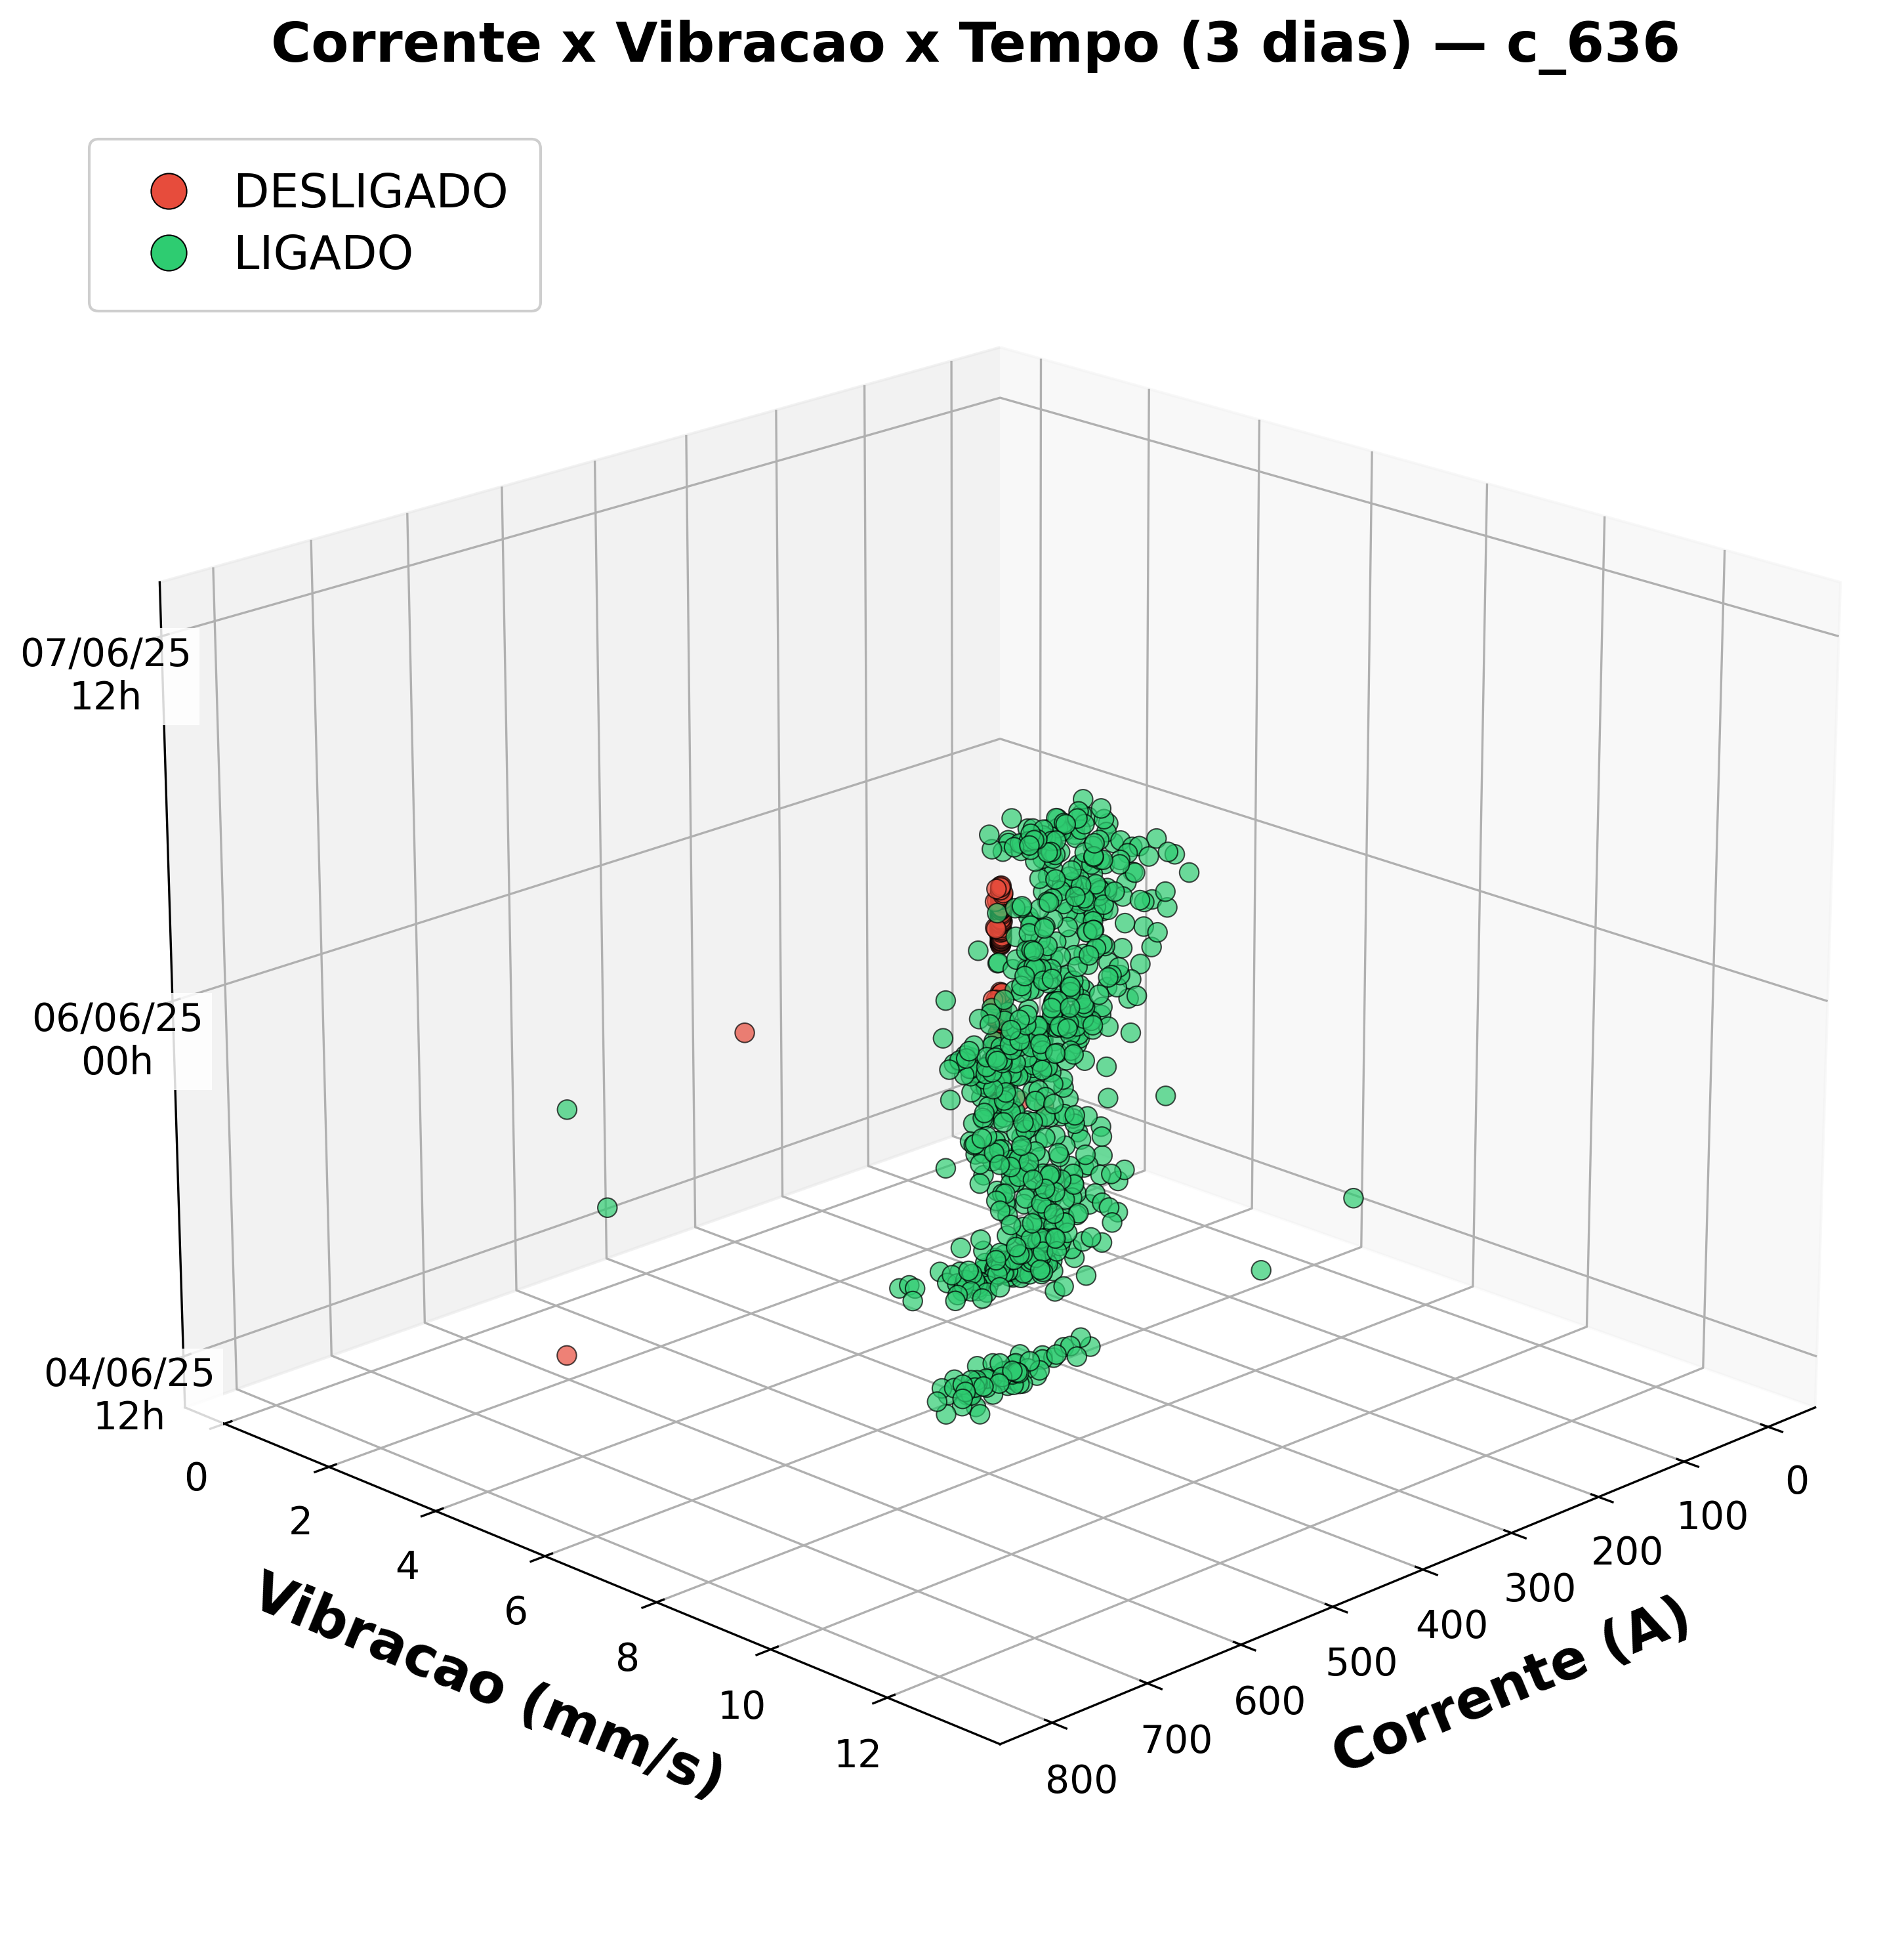
\includegraphics[width=\linewidth]{estados_corrente_vibracao_tempo_3d_c_636.png}
        \end{center}
    \end{columns}
\end{frame}

% Slide: c_1518 mecanico
\begin{frame}{Resultados: equipamento mecânico ($c_{1518}$)}
    \begin{columns}
        \column{0.6\textwidth}
        \begin{center}
            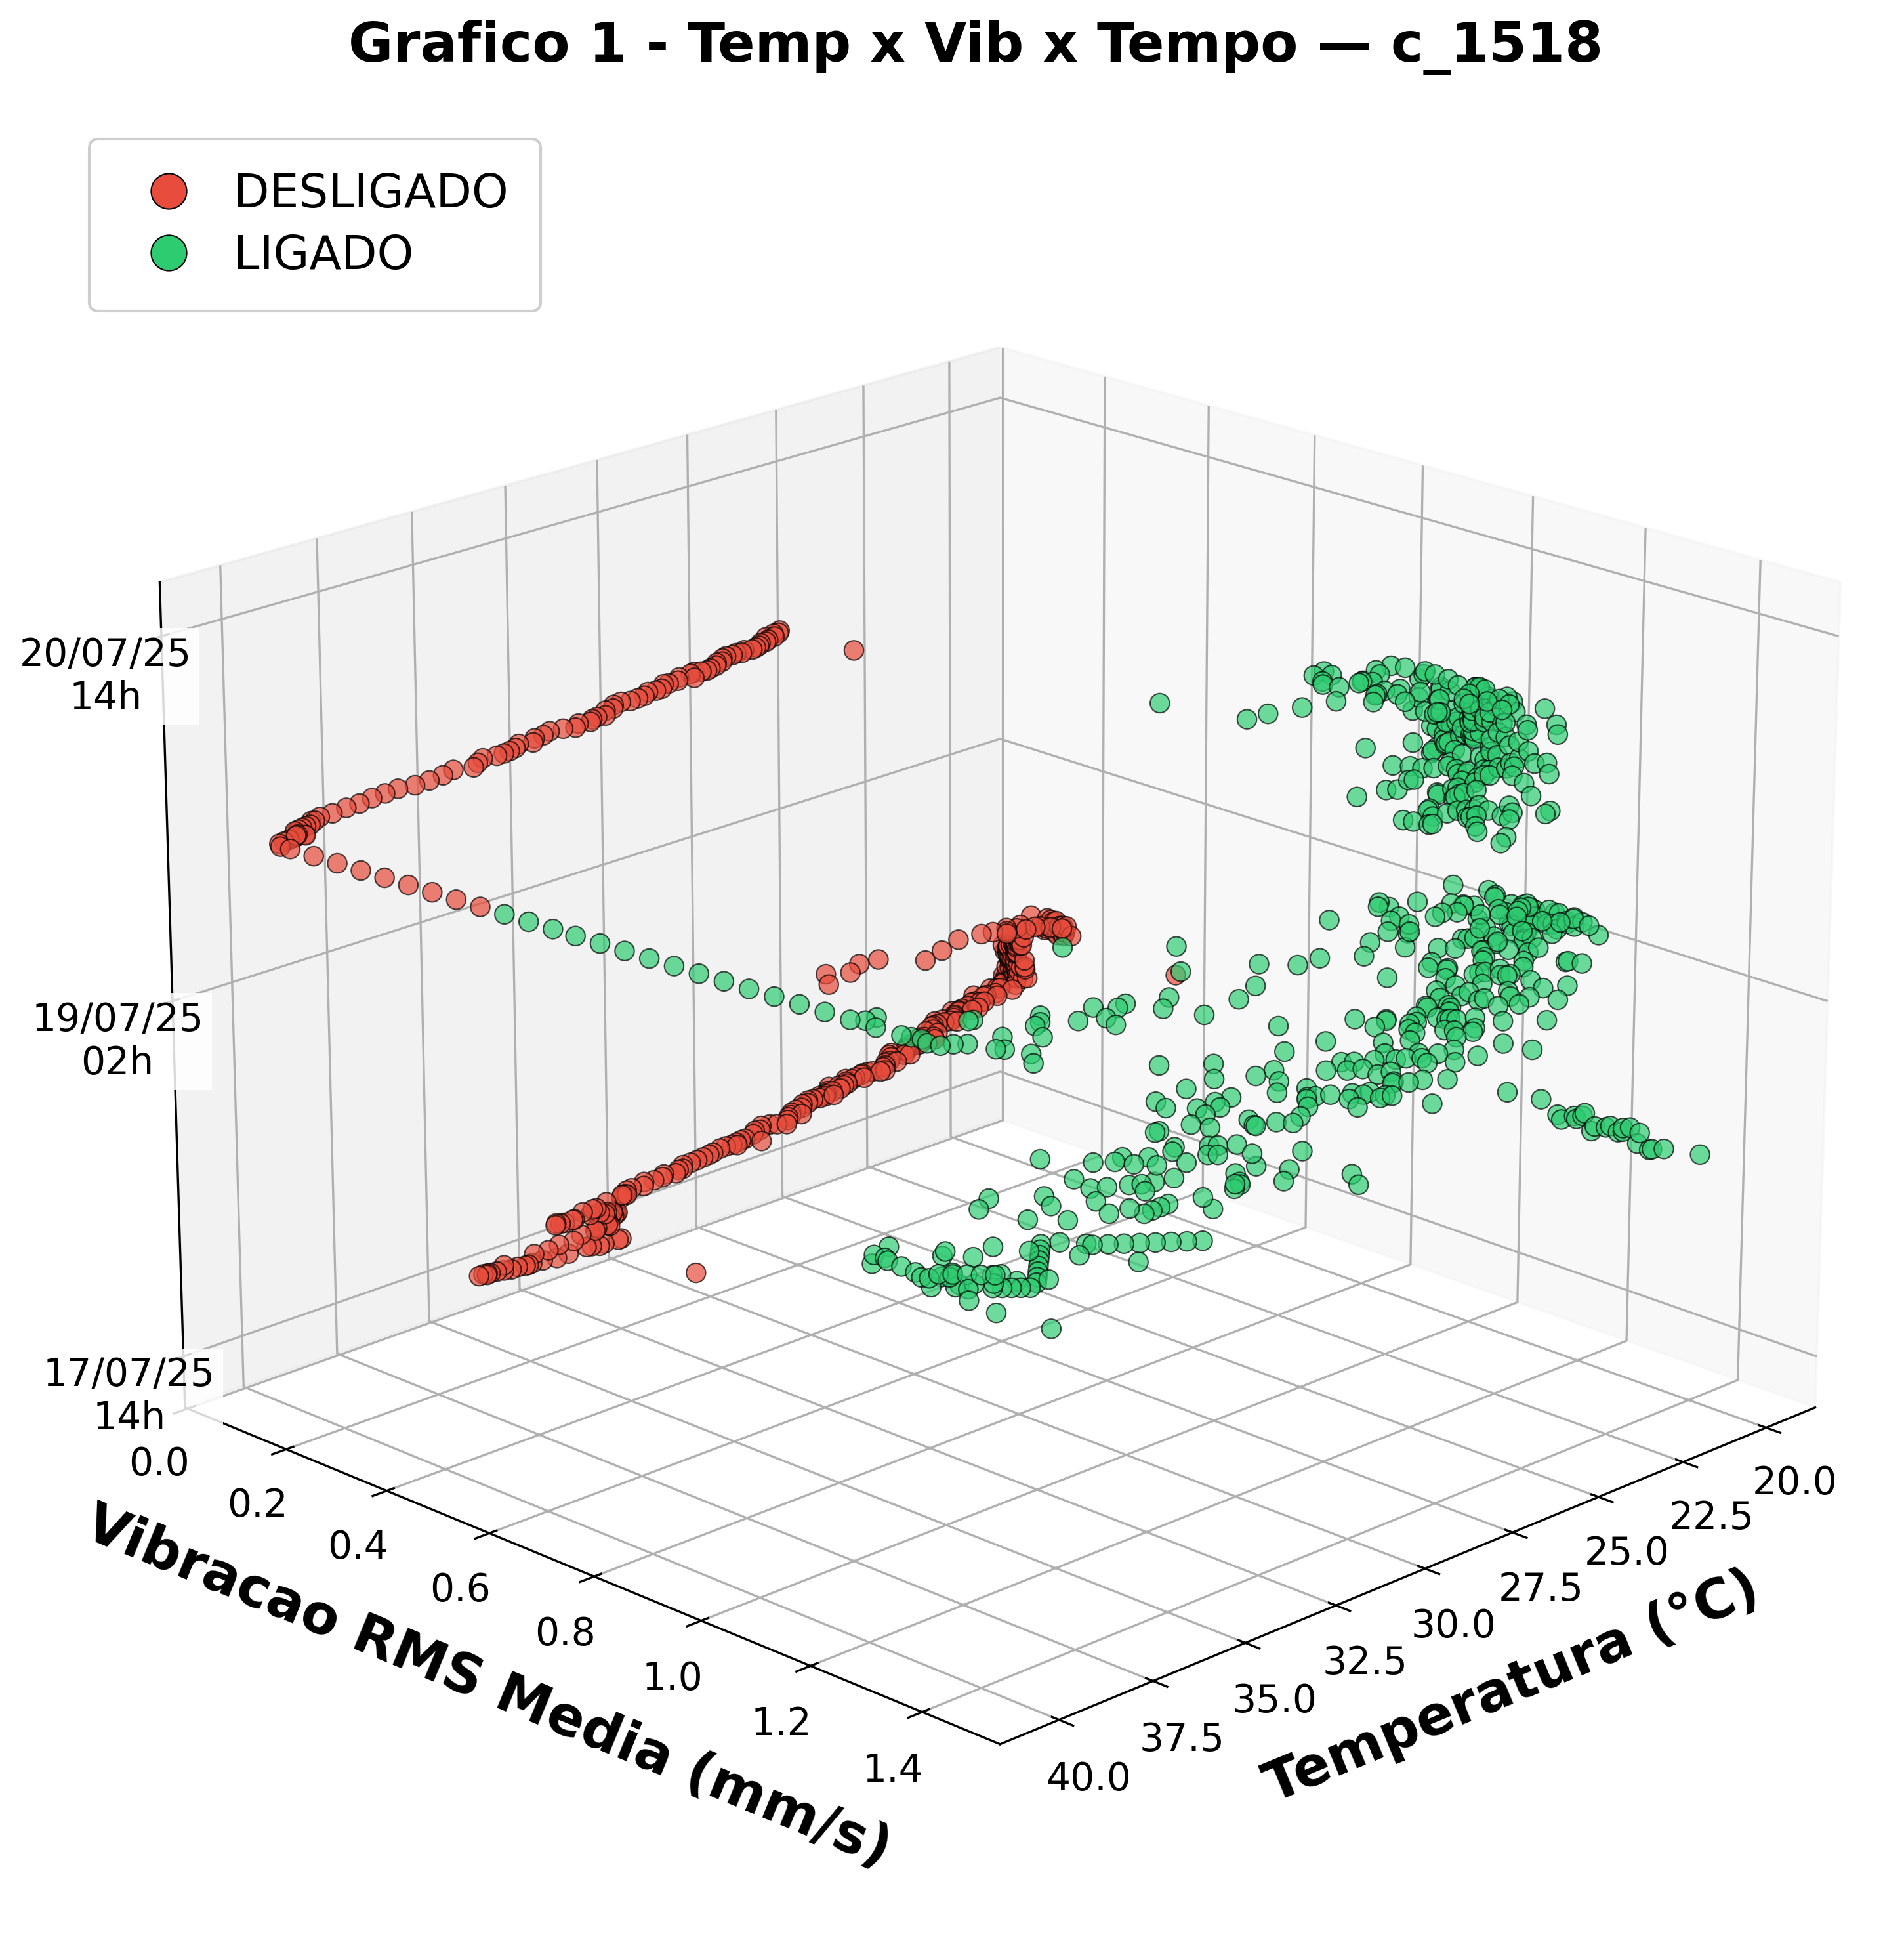
\includegraphics[width=\linewidth]{estados_temperatura_vibracao_tempo_3d_1_c_1518.png}
        \end{center}
        \column{0.4\textwidth}
        \textbf{Desafio:}
        \begin{itemize}
            \item Sem dados elétricos.
            \item Apenas temperatura e vibração.
        \end{itemize}
        \vspace{0.3cm}
        \textbf{Resultado:}
        \begin{itemize}
            \item Operação quase contínua.
            \item LIGADO 95,24\% / DESLIGADO 4,76\%.
        \end{itemize}
    \end{columns}
\end{frame}

% Slide: c_670 mecanico
\begin{frame}{Resultados: equipamento mecânico ($c_{670}$)}
    \begin{columns}
        \column{0.6\textwidth}
        \begin{center}
            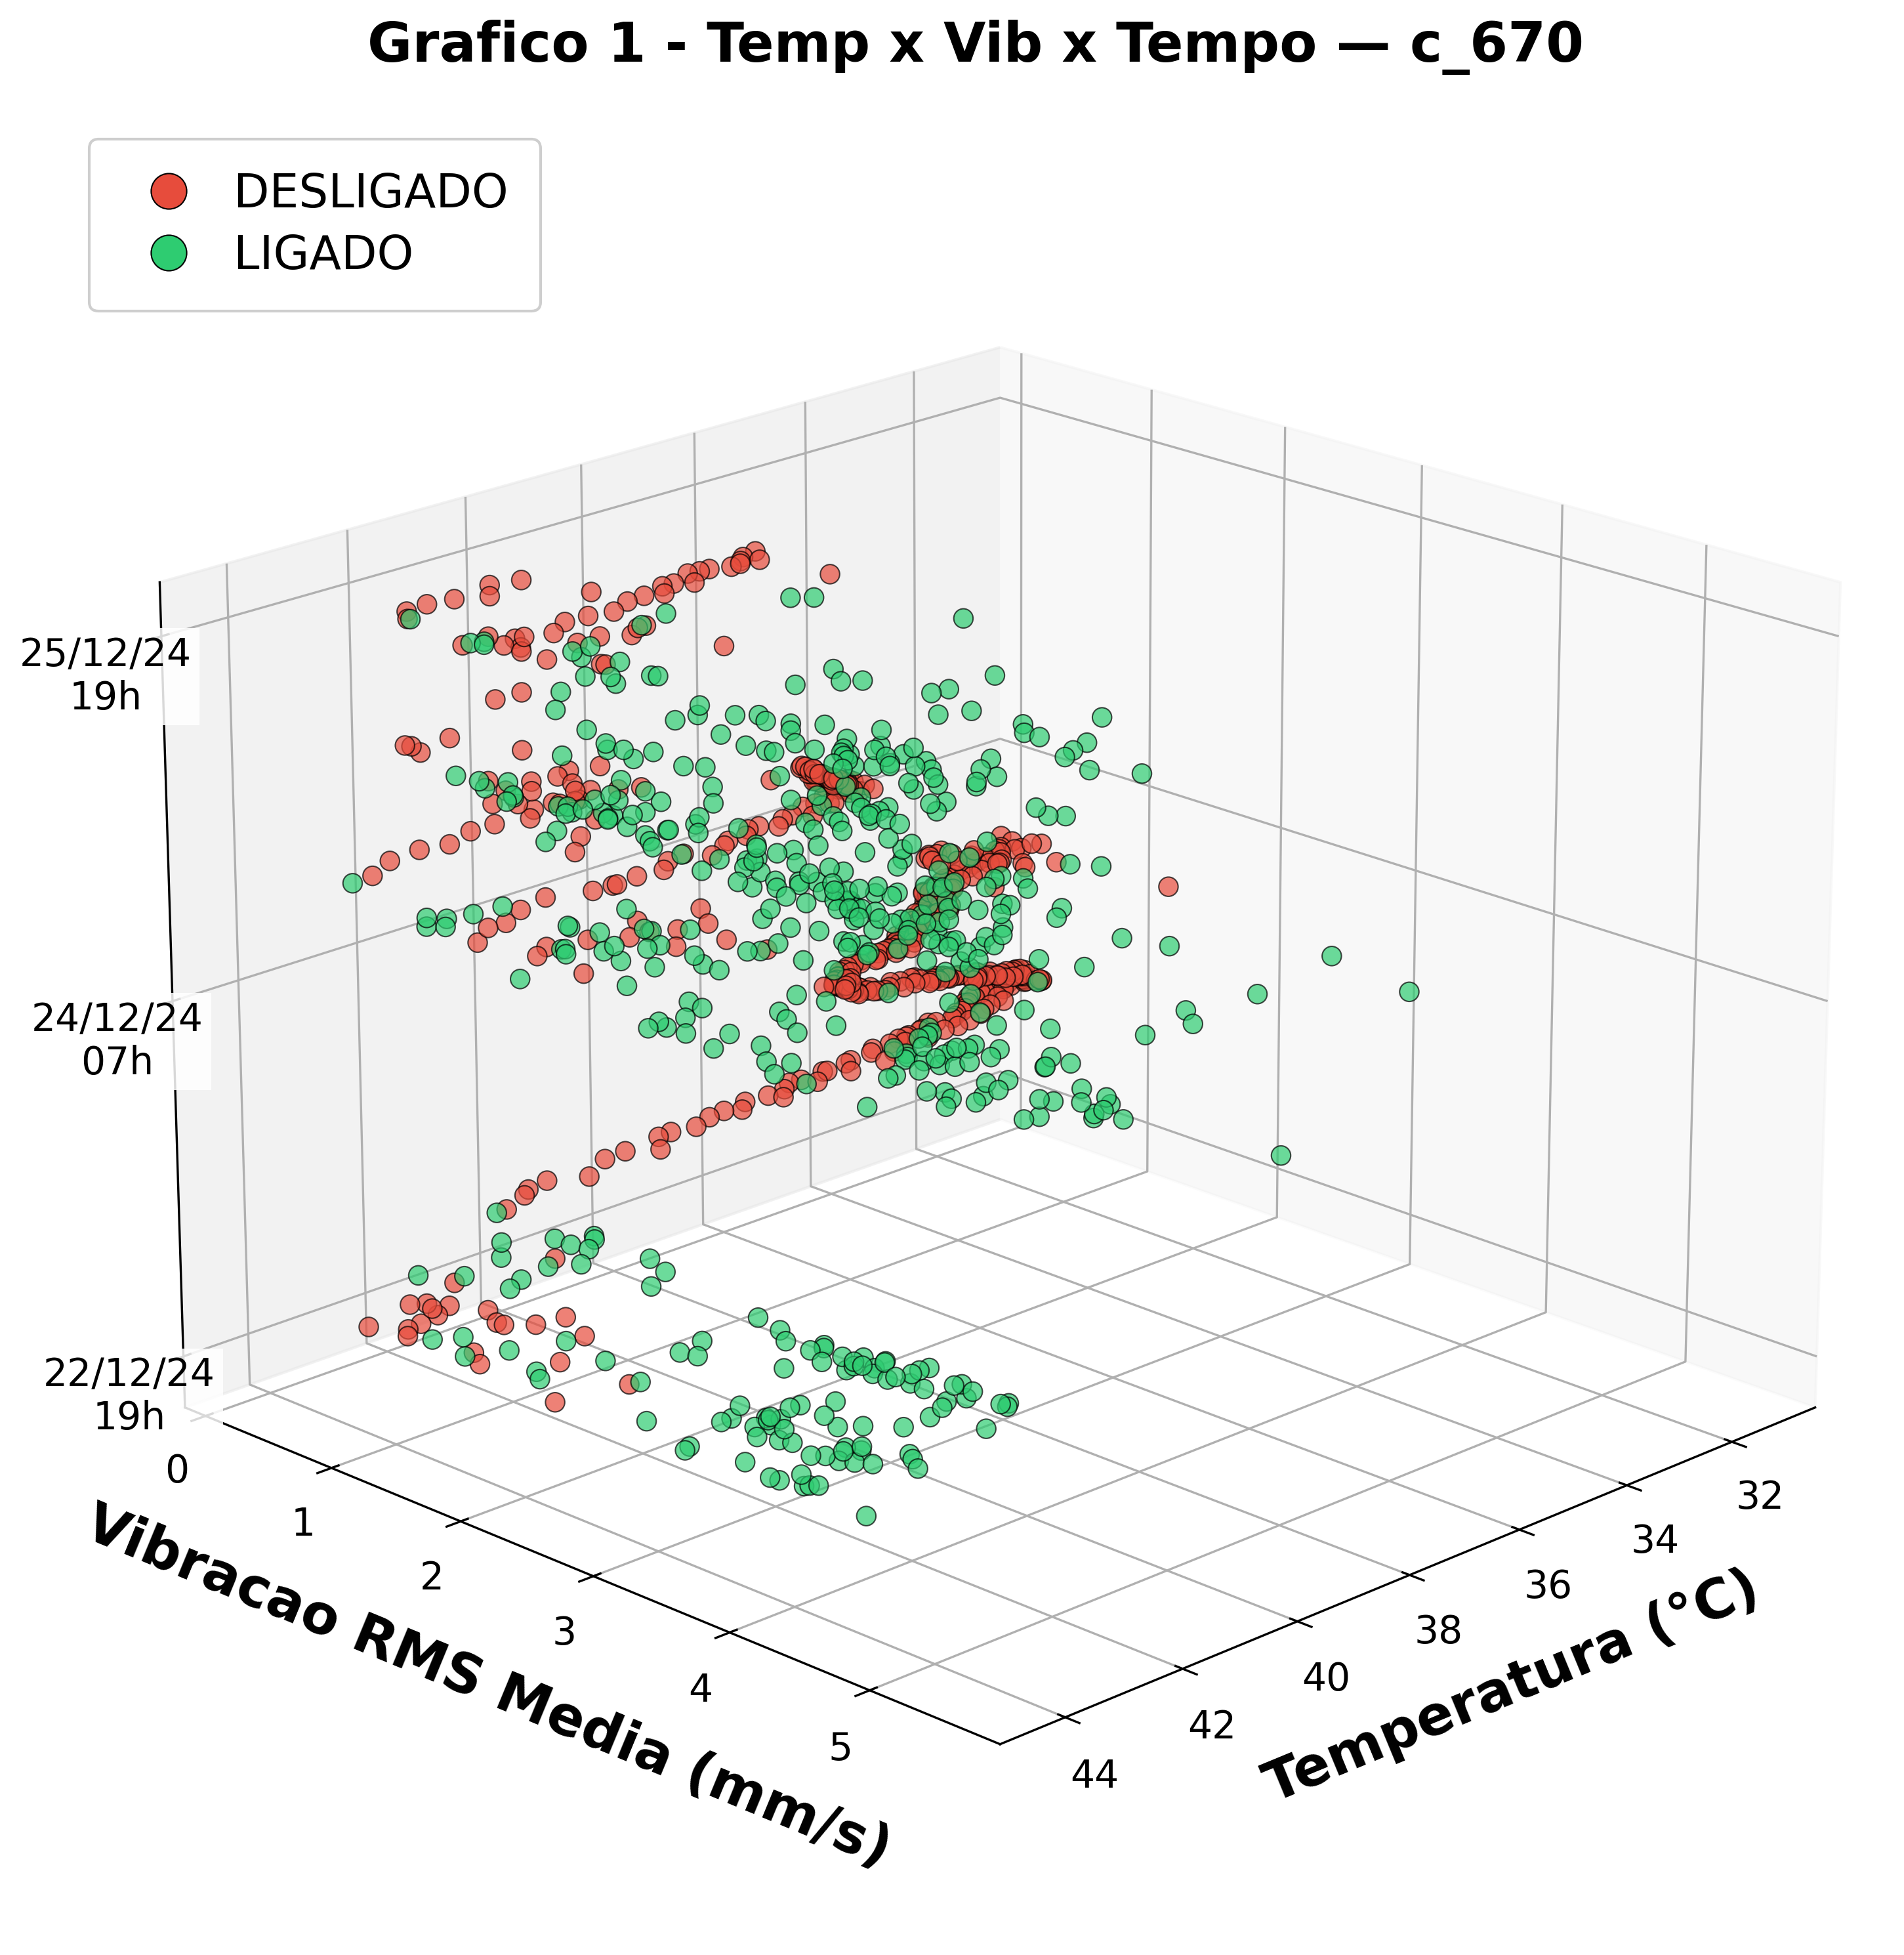
\includegraphics[width=\linewidth]{estados_temperatura_vibracao_tempo_3d_1_c_670.png}
        \end{center}
        \column{0.4\textwidth}
        \textbf{Resultado:}
        \begin{itemize}
            \item Maior proporção DESLIGADO entre os mecânicos (21\%).
            \item Discriminação clara pela \textbf{inércia térmica}: ao ligar, temperatura e vibração sobem gradualmente.
            \item No ângulo do 3D os pontos podem parecer sobrepostos.
        \end{itemize}
    \end{columns}
\end{frame}

% Slide: Reconstrucao temporal
\begin{frame}{Reconstrução temporal e horímetro}
    \begin{columns}
        \column{0.42\textwidth}
        \begin{itemize}
            \item Ciclos LIGADO/DESLIGADO ao longo de todo o histórico.
            \item Cores distinguem dado original de interpolado (PCHIP/KNN).
            \item Base para \textbf{horímetro real} e gestão de manutenção.
        \end{itemize}
        \column{0.58\textwidth}
        \begin{center}
            
\includegraphics[width=\linewidth]{vibracao_reconstrucao_c_636.png}
        \end{center}
    \end{columns}
\end{frame}

% =====================================================================
\section{Conclusão}
% =====================================================================

\begin{frame}{Conclusão e próximos passos}
    \begin{columns}
        \column{0.5\textwidth}
        \textbf{Impacto real:}
        \begin{itemize}
            \item \textbf{Gestão energética:} consumo efetivo.
            \item \textbf{Manutenção:} horímetro real vs. estimado.
            \item \textbf{Eficiência:} ociosidade não planejada.
        \end{itemize}
        \column{0.5\textwidth}
        \textbf{Trabalhos futuros:}
        \begin{itemize}
            \item \textit{Online learning} (sem re-treinar).
            \item Detecção de cavitação / operação em vazio.
        \end{itemize}
    \end{columns}
    \vspace{0.4cm}
    \begin{block}{Síntese}
        Solução simples, interpretável e escalável, validada em equipamentos elétricos e mecânicos com mais de 5,4 milhões de registros.
    \end{block}
\end{frame}

% Slide final
\begin{frame}
    \begin{center}
        {\Large Obrigado!}\\[0.6cm]
        {\large Perguntas?}\\[1cm]
        \footnotesize
        Felipe Costa Lopes --- Matrícula: 2018019648\\
        Orientadora: Profa. Gabriela Nunes --- UFMG
    \end{center}
\end{frame}

\end{document}
